\section{Ellipse Selection for Robust Pupil Detection (ElSe)}
\label{ElSe}
Zur Bestimmung der Blickrichtung ist die Augenregion natürlich von besonderer Bedeutung. Aus diesem Grund werden die Landmarks der Augenregion nochmals gesondert betrachtet. Aufgrund der besonderen Bedeutung existiert eine große Anzahl an Algorithmen, die speziell auf eine hochgenaue Bestimmung von Augenmerkmalen optimiert sind, wie Beispielsweise ElSe \cite{ElSe}, Goutam \cite{Eye_FastCorner}, Starburst \cite{Starburst} oder Swirski \cite{Swirski2012}.\\
Daher bestimmt OpenFace zusätzlich zu den 64 Landmarks, die das Gesicht beschreiben, weitere 28 Landmarks pro Auge, aus denen die Blickrichtung ermittelt wird. Um diese Augen-Landmarks zu bestimmen kommt ein weiteres CLNF zum Einsatz, das dafür trainiert wurde. Dabei zeigten die Vorabtests, dass die Detektion bei den getesteten kleinen Gesichtern unzureichend genau ausfällt.\\
Für die Bestimmung der Blickrichtung ist vor allem das Zentrum der Pupille bzw. Iris ausschlaggebend. Das Zentrum ergibt sich aus dem Umrissen (Landmarks) der Pupille bzw. Iris und muss möglichst exakt bestimmt sein., daher müssen diese aus dem Ergebnis von ElSe abgeleitet werden.\\
Um die Position der Landmarks zu verbessern, kann auf den Augenbereichen der ElSe-Algotithmus eingesetzt werden. Dieser Algorithmus basiert auf einer rechnerischen Ansatz und nicht auf Neuronen um die Umrisse der Pupille zu berechnen. Dieses Verfahren wurde gewählt, da es im Test \cite{ElSe} am besten abgeschnitten hat und direkt das Zentrum der Pupille liefert.
\subsection{Beschreibung von ElSe}
Bei realen Aufnahmen sind Bildfehler unvermeidlich, so können Reflektionen (Brille, Kontaktlinse usw.), Make-Up und körperliche Eigenschaften wie Augenfarbe die Detektion erschweren.\\
Der Ursprüngliche ElSe-Algorithmus ist für Graubilder einer Eye-Tracking-Brille ausgelegt und optimiert, zudem ist es auf diesen Bildern zu einer Echtzeitauswertung in der Lage. Dieser Anwendungsbereich betrifft vor allem die hohe Qualität der Aufnahme im Bezug auf die Auflösung und die Infrarotbeleuchtung des Bildes. Die Infrarotbeleuchtung wird verwendet, damit das Auge ausreichend beleuchtet ist ohne den Probanden zu blenden.\\
Diese Voraussetzung führen dazu, das die Detektionsleistung bei niedriger auflösenden Bildern rasch ab nimmt. Da die Berechnung unabhängig der Landmarks ausgeführt wird, empfiehlt sich das Ergebnis zu überprüfen, damit die bestimmten Landmarks auch innerhalb der Augenhöhle liegt und grobe Fehler vermieden wird.\\
Für die Anwendung wurde der ursprüngliche ElSe-Algorithmus angepasst, um auf Farbbilder die nach Grau konvertiert wurden arbeiten zu können.\\
Als Ergebnis liefert ElSe eine Ellipse, die den Umriss der Pupille im Bild beschreibt. Aus dieser Ellipse können die Landmarks der Pupille abgeleitet werden.
Ein Problem das schon im Test aufgetreten ist, entsteht wenn der Farbunterschied zwischen Iris und Pupille recht gering ausfällt oder durch Reflektionen der Kantenverlauf gestört wird.
\subsubsection{Pupille bestimmen mit Kantendetektion}
Da die Pupille als schwarzen Fleck im Bild dargestellt ist und die Iris einen helleren Farbton aufweist, wird ein Kantendetektor verwendet, der alle Pixel markiert, bei denen eine starke Farbänderung auftritt. Bei ElSe wird ein morphologischen Ansatz eingesetzt, von Relevanz sind nur zusammenhängende Kantenpixel um die Kante zwischen Pupille und Iris zu finden. Alle anderen Pixel können ignoriert werden, wobei jedes Kantenpixel als Startpunkt der Berechnung dienen kann.\\
Um jene Kantenpixel zu erhalten, die die Pupille beschreiben, wird versucht fortlaufende Kanten zu finden, die eine Ellipse bilden. Jene die nicht diesen Anforderung entsprechen, können recht schnell ignoriert werden. Anschließend werden auch alle offenen Ellipsenverläufe und jene Kantenpixel die am meisten vom bestimmten Verlauf abweichen, verworfen.\\
Das beste Ergebnis aller bestimmten Ellipsen wird als Lösung verwendet.
\subsubsection{Grobe Bestimmung der Pupille}
\label{ElSe_Grob}
Sollte die Bestimmung der Ellipse, wie im letzten Kapitel beschreiben, scheitern, so wird das Zentrum des dunkelsten Kreises ermittelt. So ein Punkt kann immer gefunden werden, ist aber nicht zwingend die Pupille.\\
Auf einem verkleinertem Bild \autoref{img_else} (1) wird ein kreisförmiger Mean-Filter eingesetzt mit Ergebnis in \autoref{img_else} (3). Zur zweiten Faltung wird der Durchschnitt über ein Quadrat ohne inneren Kreis eingesetzt mit Ergebnis in \autoref{img_else} (2), wobei bei beiden Kreisen der selbe Radius verwendet wird.\\
Nun wird das Ergebnis des Quadratischen Mean-Filters invertiert \autoref{img_else} (4) und mittels Punkt-Multiplikation mit dem anderen Meanfilter zusammengebracht \autoref{img_else} (5). Im resultierendem Bild wird nun der höchste Wert gesucht, da dies das Zentrum des dunkelsten kreisförmigen Ortes im Bild ist.\\
Ergebnis des Beispiels ist als Kreuz in \autoref{img_else} (6) markiert. 
\begin{figure}
	\centering
	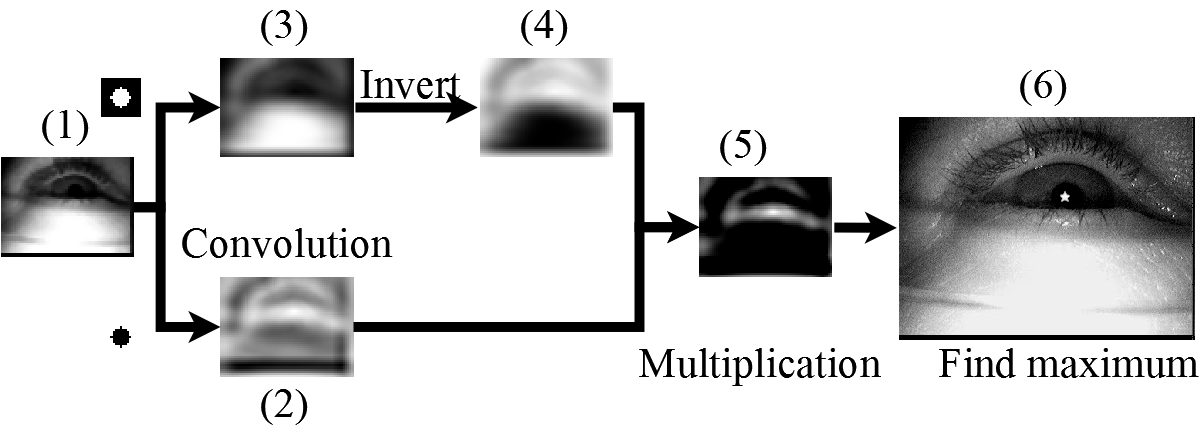
\includegraphics[width=0.8\linewidth]{img/ElSe}
	\caption{Ablauf der alternativen Berechnung zur Pupillen-Detektion von \cite{ElSe}}
	\label{img_else}
\end{figure}
\subsubsection{Veröffentlichte Ergebnisse}
Für den Test, wurden Bilder von $384\times 288$ Pixel Größe verwendet.
Im Vergleich zu den anderen Verfahren, ist ElSe in den meisten Fällen überlegen, mit einer Verbesserung der Erkennungsrate um $14.53\%$ auf dem verwendeten Datensatz \cite{ElSe}.
\subsection{Das Verfahren im Test}
Der Ursprüngliche ElSe-Algorithmus wurde für Eye-Tracking Brillen entwickelt worden, daher soll geprüft werden in wieweit es in dieser Anwendung eingesetzt werden kann.\\
Um die einzelnen Grau-Verfahren besser Vergleichen zu können, wurden künstliche Augen aus dem Datensatz \cite{database_Eye} verwendet damit die exakte Position der Landmarks bekannt ist.\\
Ein gutes Verfahren muss stabil gegenüber der Skalierung sein, damit es auch auf kleinen Bereichen zuverlässig arbeitet. Da für die spätere Anwendung vor allem das Zentrum der Pupille von Interesse ist, wird der euklidische Abstand zum Zentrum als Qualitätsmaß verwendet.\\
Da ElSe für Eye-Tracking Brillen entwickelt wurde, also für ein Qualitativ hochwertiges Bild eines Auges, wurde der Bildbereich soweit verkleinert das nur noch alle Landmarks des Auges mit etwas Rand dargestellt werden, um diesen Anforderungen entsprechend nahe zu kommen.\\
Somit sind die Bildausschnitten im Datensatz auf denen gerechnet wird etwa 64 auf 29 Pixel groß und werden für die Verarbeitung auf eine Breite von 384 Pixeln vergrößert, die Auflösung, wofür ElSe entwickelt wurde. Da durch die Skalierung allerdings keine zusätzlichen Informationen entstehen, ist vor allem die grobe Bestimmung der Ellipse, beschreiben in \autoref{ElSe_Grob}, von Interesse. Diese Auswahl des Bildbereiches kann auch in der späteren Anwendung eingesetzt werden, da der Augenbereich durch eigene Landmarks in der Gesichtsanalyse, relativ genau bestimmt ist.\\
Um die Qualität der Berechnung bei verschiedenen Größen zu ermittelt, wurde das Bild linear verkleinert.
\subsubsection{Auswirkung der verschiedenen Graubild-Verfahren}
Es zeigt sich, dass die Verfahren, um den Farbwert in einen Grauwert zu überführen, durchaus Auswirkungen auf die Qualität der Berechnung hat.\\
Als Kriterien wird die Differenz zwischen den berechneten Radien der den Datensatzes von der Pupille und Iris. Außerdem der euklidischen Abstand zum berechneten Zentrum der Pupille.\\
Der minimale Abstand der Berechneten Zentren ergibt sich bei dem Gleam-Verfahren mit $5.327$ Pixel als Median, siehe \autoref{img_vergleich_A}. Der Beste Radius für den Filter ist für die Position der Iris bei 10 Pixel\\
Ein Unterschied zwischen den Verfahren konnte bei der Bestimmung des Radius der Pupille nicht gefunden werden, siehe \autoref{img_vergleich_PI} links. Der beste Radius für den Filter ist im Test bei 8 Pixel und ergibt eine Abweichung von $1,555$ Pixel.\\
Für die Bestimmung der Iris hat das quadratische Verfahren die geringste mittlere Abweichung mit $2,488$ Pixel, nur etwas genauer als Min-Verfahren ($2,49$ Pixel). Für diese Berechnung ist ein Radius des Filters von 18 Pixel am besten gewählt.\\
Somit wurde drei Verfahren ausgewählt um diese näher zu untersuchen, Gleam mit der geringsten Abweichung des Zentrums, Quadrat als bestes Resultat bei der Iris und Luminance da es ein Standartverfahren ist. Alle mit den Radien $8/10/18$ für die Berechnung der Pupille/Zentrum/Iris.\\
Es zeigt sich, das der Fehler in den Berechnungen über einen großen Skalierungsbereich gleich bleibt. Der Fehler bei der Bestimmung des Zentrums ist bis zu einer Skalierung von $0,4$ bei $5,4$ Pixel, siehe \autoref{img_Vergleich_Scal_A}.\\
Auch bei der Berechnung der Pupille ist weiterhin kein Unterschied zu erkennen, siehe \autoref{img_Vergleich_Scal_PI} oben.\\
Die Bestimmung der Pupille und Iris bleibt auf dem glichen Niveau bis zu einer Skalierung von $0,15$. Auch bleibt die Unterschiede der Verfahren bleiben immer ähnlich.
\begin{figure}
	\centering
	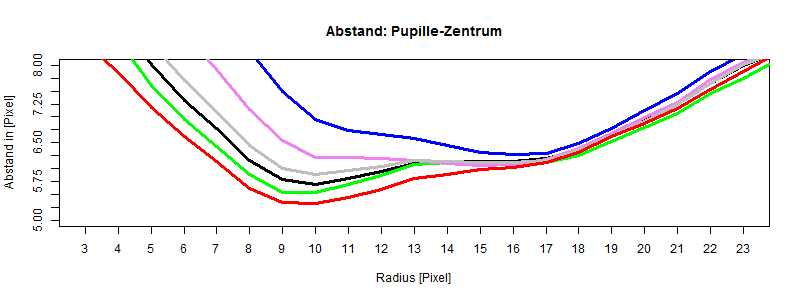
\includegraphics[width=\linewidth]{Eye_Img_Box/Vergleich_A}
	\caption{Median-Abstand in Pixel des Zentrums der Pupille gegen die Veränderung des Radius des Filters.\\
	Verfahren: Gleam (rot), Luminance (schwarz), Max (grün), Min (violett), New-Gleam (grau), Quadrat (blau)}
	\label{img_vergleich_A}
\end{figure}
\begin{figure}
	\centering
	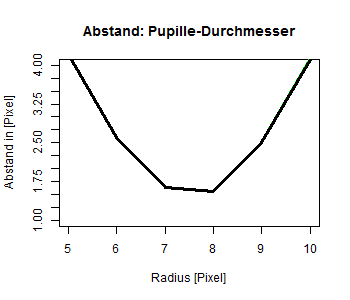
\includegraphics[width=0.49\linewidth]{Eye_Img_Box/Vergleich_P}
	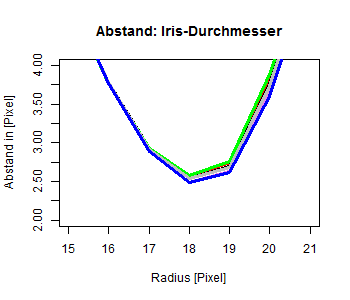
\includegraphics[width=0.49\linewidth]{Eye_Img_Box/Vergleich_I}
	\caption{Differenz zwischen den Radien gegen die Veränderung des Radius des Filters von Pupille (links) und Iris (rechts)\\
	Verfahren: Gleam (rot), Luminance (schwarz), Max (grün), Min (violett), New-Gleam (grau), Quadrat (blau)}
	\label{img_vergleich_PI}
\end{figure}
\begin{figure}
	\centering
	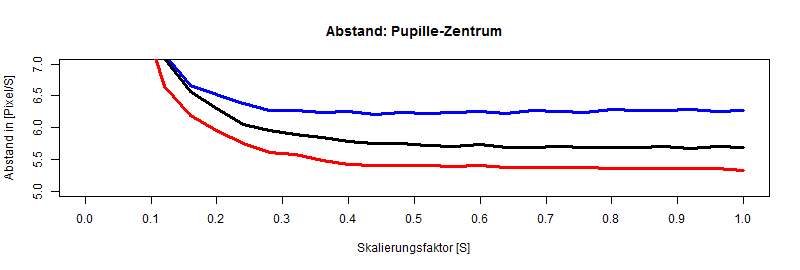
\includegraphics[width=\linewidth]{Eye_Img_Box/Vergleich_Scal_A}
	\caption{Euklidischer Abstand in Pixel zwischen dem berechneten Zentrum der Pupille und dem des Datensatzes gegen die Veränderung des Radius des Filters.\\
		Verfahren: Gleam (rot), Luminance (schwarz),  Quadrat (blau)}
	\label{img_Vergleich_Scal_A}
\end{figure}
\begin{figure}
	\centering
	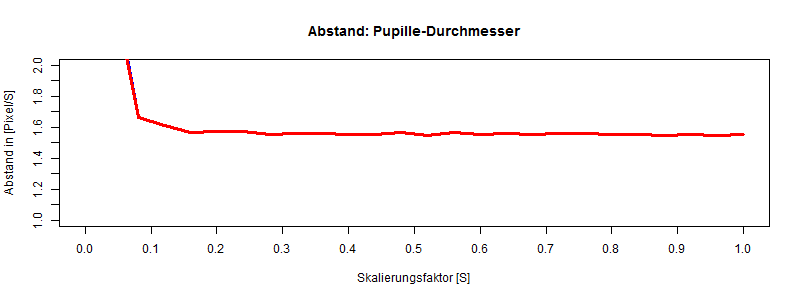
\includegraphics[width=\linewidth]{Eye_Img_Box/Vergleich_Scal_P}
	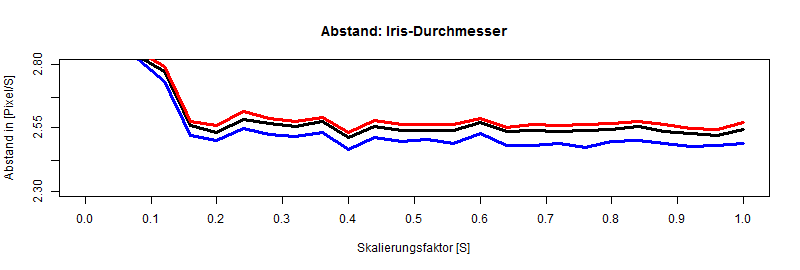
\includegraphics[width=\linewidth]{Eye_Img_Box/Vergleich_Scal_I}
	\caption{Differenz in Pixel zwischen den Radien der Berechnung und dem des Datensatzes gegen die Veränderung des Radius des Filters. Oben: Pupille, Unten Iris\\
		Verfahren: Gleam (rot), Luminance (schwarz), Quadrat (blau)}
	\label{img_Vergleich_Scal_PI}
\end{figure}
\subsubsection{Auswirkung des Filterradius}
Ein wichtiger Parameter des ElSe-Verfahrens ist der Radius des Filters. Um den besten Parameter zu bestimmen wurde der Augen-Datensatz \cite{database_Eye} verwendet und die Augenpartie ausgeschnitten. Im Datensatz besitzen die abgebildeten Augen durchschnittlich 15 Pixel Breite Pupille und eine Iris von 34 Pixel Durchmesser.\\
In \autoref{img_vergleich_PI} ist zu erkennen, dass der Radius signifikant für die Qualität der Berechnung ist. Da für die spätere Anwendung vor allem das Zentrum der Pupille von Interesse ist, vgl. \autoref{OpenFace_Blickrichtung}, muss ElSe in diesem Aspekt zuverlässig Ergebnisse liefern.\\
Im Versuch hat sich ein Radius von etwa einem Zwölftel des zu erwartetem Durchmesser der Iris bzw. Pupille als sinnvoll erwiesen, um deren Ausmaße möglichst exakt zu bestimmen. Im Versuch entspricht dies 8 und 18 Pixel.\\
Um die Position des Zentrums der Iris und der Pupille möglichst gut zu bestimmen, erwies sich ein Radius von 10 am besten, siehe \autoref{img_vergleich_A}, wobei dieser Fehler nicht so sehr steigt bei Veränderung des Radius, als bei der Größenbestimmung von Pupille und Iris.
\subsubsection{Vergleich zu OpenFace}
Als Referenz wird das Ergebnis von OpenFace, für die zusätzlich bestimmten Landmarks der Augen, verwendet. Dies wurde auch auf dem Augendatensatz \cite{database_Eye} angewendet, um vergleichbare Ergebnisse zu erhalten.\\
In \autoref{OpenFace_Eye} ist zu erkennen dass dieses Verfahren im Schnitt oft schlechtere Ergebnisse liefert als das ElSe, allerdings ohne großen Fehler und auch öfters genauere Ergebnisse.\\
Da die hohe Qualität von ElSe nur erreicht werden kann, wenn es auf passenden Bildausschnitt angewendet wird, ist auch die Detektion des Auge von Interesse.\\
Nach \autoref{OpenFace_Eye_Box} ist zu entnehmen, dass der Bereich des Auges zwar nicht so exakt bestimmt wird, allerdings überdeckt er den relevanten Bereich ausreichend genau. Somit liegen die Landmarks der Augen im Bildausschnitt, wodurch diese Ausschnitt als Eingabe von ElSe verwendet werden kann.
\begin{figure}
	\centering
	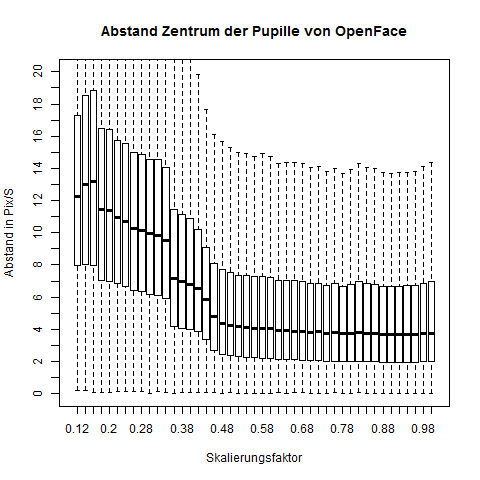
\includegraphics[width=0.45\linewidth]{Eye_Img_Box/Openface_PC}
	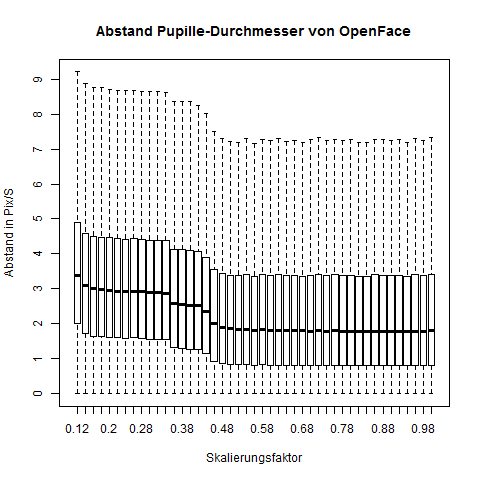
\includegraphics[width=0.45\linewidth]{Eye_Img_Box/Openface_PW}
	%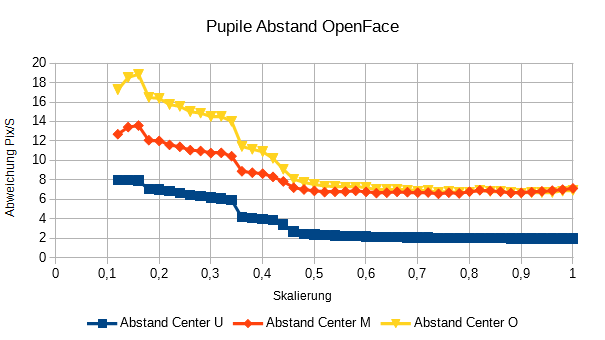
\includegraphics[width=0.45\linewidth]{Eye_Img/OpenFace_Zentrum_P}
	%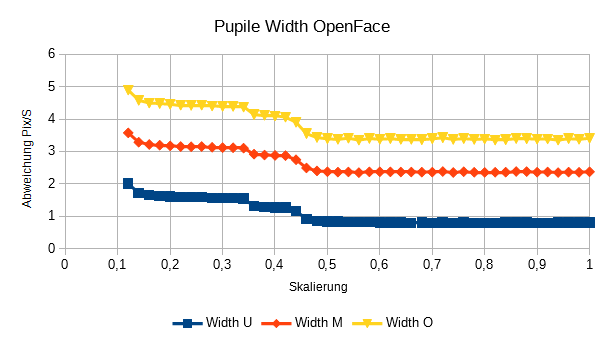
\includegraphics[width=0.45\linewidth]{Eye_Img/OpenFace_Width_P}
	\caption{Auswirkung der Bildgröße auf die Qualität der Augendetektion von ObenFace. Aufgetragen ist die Abweichung [Pixel/Skalierung] gegen den Skalierungsfaktor.}
	\label{OpenFace_Eye}
\end{figure}
\subsection{Ergebnis}
Im Test ist bei allen Skalierungen im durchschnitt ElSe den Ergebnisse von OpenFace überlegen, durch die Verteilung ist allerdings eine Kombination beider Verfahren sinnvoll, so kann das Ergebnis von OpenFace bei Bilder in denen die Iris größer als 21 Pixel ist direkt als Lösung verwendet werden, da der mögliche Fehler von OpenFace geringer ist als der von ElSe.\\
Im Bereich zwischen 21 und 15 Pixel können beide Ergebnisse Kombiniert werden, da sie ungefähr gleich gute Ergebnisse liefern.\\
Sollte die Iris im Originalbild noch kleiner sein, so ist ElSe deutlich genauer, da es noch bis zu einer Irisgröße von 3 Pixel stabil funktioniert.\\
Es ist zu erkennen, das ElSe zwar oft bessere Ergebnisse liefert als OpenFace, wobei auch grobe Fehler auftreten können, was an der Verteilung zu erkennen ist wenn \autoref{OpenFace_Eye} und \autoref{ElSe_scall} verglichen werden.
Eine genauere Darstellung der Messergebnisse ist in \autoref{Abbildungen} dargestellt. Die Auswirkung der Radien und der verschieden Verfahren auf die Pupille ist in \autoref{ElSe_Gray_Pupille}, auf die Iris in \autoref{ElSe_Gray_Iris} und auf die Bestimmung des Zentrums in \autoref{ElSe_Gray_Zentrum}. Die Auswirkung der Skalierung in \autoref{ElSe_scall}.